\documentclass[10pt,a4paper]{article}
%\special{papersize=297mm,210mm}
\usepackage[landscape,twocolumn,margin={2cm,2cm}]{geometry}
\setlength{\columnsep}{16mm}

\usepackage[utf8]{inputenc}
\usepackage[T1]{fontenc}
%\usepackage{PTSans}
\usepackage{tgtermes} %times
\usepackage[scaled]{uarial}
\usepackage{sectsty} %change font on headings
\allsectionsfont{\sffamily}

\usepackage{multirow}
\usepackage[hidelinks]{hyperref}
\usepackage{enumitem}
\usepackage{graphicx}
\usepackage{pdfpages}
\usepackage{rotating}
\usepackage{adjustbox}
\usepackage{epstopdf}

\title{\bf\sffamily\fontsize{18}{18}\selectfont{
Course Program\\ ETS170 Requirements Engineering\\http://cs.lth.se/ets170 
}}
\author{\bf\sffamily\fontsize{12}{12}\selectfont{Björn Regnell, Elizabeth Bjarnason}}
\date{\bf\sffamily\fontsize{10}{10}\selectfont{Study period: 2016-HT2, Revision date: \today}}
\begin{document}

\maketitle
\noindent 
The objective of the course is to give basic and advanced knowledge and skills within requirements engineering for large-scale development of systems completely or partly based on software. The course gives both theoretical knowledge and practical skills in methods and techniques for requirements engineering. The course gives training in scientific paper reading.

\section{Learning Objectives}
\subsection{Knowledge and understanding}
For a passing grade the student must
\begin{enumerate}[noitemsep]
\item be able to define basic concepts and principles within requirements engineering 
\item give an account of several different types of requirements
\item be able to describe and value several different methods and techniques for requirements engineering
\item be able to describe and relate different sub-processes within requirements engineering
\item be able to describe the relation between the requirements engineering process and other processes in the product lifecycle
\item be able to describe the relation between requirements engineering and market-driven product management
\item be able to discuss some scientific results within requirements engineering research
\end{enumerate}


\subsection{Skills and abilities}
For a passing grade the student must
\begin{enumerate}[noitemsep]
\item be able to choose suitable requirements techniques for a given context
\item     be able to apply several different techniques for requirements elicitation
\item     be able to apply several different techniques for requirements specification
\item     be able to apply several different techniques for requirements validation
\item     be able to apply several different techniques for requirements prioritisation
\end{enumerate}
  The release plan defines which requirements that are implemented by the development team as mock-up designs in release R3, and which requirements are selected to be fully implemented in the imagined releases R4 and R5. 
\subsection{Judgement and approach}
For a passing grade the student must
\begin{enumerate}[noitemsep]
\item     be able to consciously select a process depending on the nature of the requirements
\item     show a systematic and long-term approach to processes
\item     be able to consciously see the problem in the relation between the quality of requirements and the quality of the resulting implementation
\item     be able to adequately involve users in the requirements engineering process
\item     be able to consciously see the problem in the relation between requirements engineering and economical aspects of product development
\end{enumerate}

\section{Contents}
The course includes theory and practice regarding the following topics:
\begin{enumerate}[noitemsep]
\item Requirements on different abstraction levels and in different contexts

\item Sub-processes of requirements engineering and their relation

\item Specification of data requirements, e.g. using virtual windows and data models

\item Specification of functional requirements, e.g. using textual feature requirements and task descriptions

\item Specification of different types of non-functional requirements, e.g. usability, performance, reliability

\item Different techniques for requirements elicitation

\item Different techniques for requirements validation

\item Different techniques for requirements prioritization

\item Market-driven requirements engineering and product management
\end{enumerate}

\newpage

\section{Course elements}
\begin{description}
\item[L: Lectures] The lectures provide an overview of the literature. They do not cover every detail, but give a high-level structure of the subject and thereby aid self-studies of the literature. Discussions are promoted.
\item[E: Exercises] The main objective of the exercises is to support the project and prepare for the written exam through prototypical problems, by connecting theory to practice and to give opportunity to discuss details of RE techniques.
\item[LAB: Computer lab sessions] The lab sessions illustrate computer supported
prioritization and release planning, and demonstrates the complexity of requirements selection and scheduling. Preparations are mandatory. 
\item[P: Project] The project is carried out in groups of 6-8 students. The project involves a number of deliverables and a final project conference where the learning outcome of each project is presented. Project groups are established during the first course week. Project assignments are established during the second course week.
\end{description}




\section{Assessment}
\begin{itemize}
\item The project is graded fail/3/4/5 based on project deliverables.
\item Approved lab session preparations and assignments are required for passing.
\item The written exam comprises 100 points. The pass limit is 50 points.
\item It is optional to hand in two sets of candidate exam problems. Good candidate exam problems can give a maximum of 10 bonus points added to the result of the written exam if they are handed in before stipulated deadlines. The bonus can be used at written exams within 10 months after the course ending.
\item The final course grade on the scale fail/3/4/5 is based on the written exam points including bonus and the project grade using the following mapping:

\begin{tabular}{r | c c c}
 & Project: 3 & Project: 4 & Project: 5 \\
\hline
 & \multicolumn{3}{c}{Exam points + bonus}    \\
Final: 3 & $ \geq 50$ & $\geq 50$ & $\geq 50$ \\
Final: 4 & $ \geq 75$ & $\geq 67$ & $\geq 60$ \\
Final: 5 & $ \geq 90$ & $\geq 83$ & $\geq 75$ \\
\hline
\end{tabular}


\end{itemize}


\section{Literature}
The course elements and the written exam will cover the following literature: 
\begin{flushleft}
\setlength{\tabcolsep}{0pt}
\begin{tabular}{p{0.15\columnwidth} p{0.85\columnwidth}}
Lau & Soren Lauesen, Software Requirements - Styles and Techniques, Addison-Wesley, ISBN 0-201-74570-4, 2002. \\
LAB1\&2	&Preparations and instructions for Lab 1: ''Requirements Modeling'' and Lab 2: ''Requirements Prioritization and Release Planning'' \\
MDRE &	''Market-Driven Requirements Engineering for Software Products'', Björn Regnell and Sjaak Brinkkemper, Engineering and Managing Software Requirements, Eds. A. Aurum and C. Wohlin, Springer,  ISBN 3-540-25043-3, 2005 \\
PRIO&	''Requirements Prioritization'', Patrik Berander and Anneliese Andrews, Engineering and Managing Software Requirements, Eds. A. Aurum and C. Wohlin, Springer,  ISBN 3-540-25043-3, 2005 \\
OSSRE & ''Understanding Requirements for Open Source Software'', Walt Scacchi, Design Requirements Engineering: A Ten-Year Perspective, Springer, pp. 467-494, 2009\\
 RP&	''The Art and Science of Software Release Planning'', Günther Ruhe and Moshood Omolade Saliu, IEEE Software, November/December, pp. 47-53, 2005  \\
QUPER&	Supporting Roadmapping of Quality Requirements - Björn Regnell, Richard Berntsson Svensson, 
Thomas Olsson, IEEE Software 25(2) pp 42-47 March-April 2008  \\
INSP&	''Att inspektera krav''. Sid 67-76, Framgångsrik kravhantering, andra utgåvan, Teknikföretagen, Joachim Karlsson, V040072, ISSN 1103-7008, 1998\\
 INTDEP &	''An industrial survey of requirements interdependencies in software product release planning'', Carlshamre, P., Sandahl, K., Lindvall, M., Regnell, B., Natt och Dag, J.: Int. Conf. on Requirements Engineering (RE01), Toronto, Canada, pp. 84–91, 2001 \\
AGRE &	''Agile Requirements Engineering Practices: An Empirical Study'', Lan Cao, Balasubramaniam Ramesh, IEEE Software , January/February 2008, pp.60-67, 2008 \\
\end{tabular}
\end{flushleft}

\newpage
\section{Overview}

\begin{flushleft}
\small
\begin{tabular}{c | p{0.5cm} p{4.4cm} p{2.2cm}  p{3.2cm}}
 &  & {\it Topic} & {\it Literature} & {\it When}   \\
\hline
\multirow{4}{*}{\rotatebox{90}{\bfseries\sffamily Week 1}} 
 & L1 & Introduction BR & Lau:1 & Mon 10-12\\
 & E1 & Requirements types &  Lau:1  & Mon 15-17 or Wed 8-10\\
 & L2 & Elicitation, Specification 1 BR & Lau:8,2-3.5& Th 10-12\\
 & P  & Project Mission v1 -> BR EB AO &  & Deadline Fri 09:00 \\
\hline
\multirow{4}{*}{{\bfseries\sffamily W2}} 
 & L3 & Spec 2, Mission lottery AO & Lau:3.6-4 & Mon 10-12\\
 & E2 & Elicitation  & Lau: 8  & Mon 15-17 or Wed 8-10\\
 & P & Meeting with supervisor & & \\
 & reqT & reqT \& Scala tutorial - BR & \href{http://reqt.org}{reqT.org} & Thu 10-12 \\
\hline
\multirow{4}{*}{{\bfseries\sffamily W3}} 
 & P  & Project Mission v2 -> supervisor&  & Mon 09:00 \\
 & L4 & Market-driven + Open Source RE, Prio, Rel Plan JL & MDRE, PRIO, RP, OSSRE & Mon 10-12\\
 & E3 & Functional requirements  & Lau:2-4  & Mon 15-17 or Wed 8-10\\
 & Lab1 & Requirements Modelling & LAB1 &  Wed 13-15 or 15-17 or Thu 8-10 or 10-12\\
\hline
\multirow{3}{*}{{\bfseries\sffamily W4}} 
 & P & Release R1 -> supervisor& & Deadline Mon 09:00 \\
 & P & Meeting with supervisor & & \\
 & L5 & Specification 3, Quality, Lifecycle & Lau:5-7, QUPER  & Mon 10-12\\
 & E4 & Quality requirements &  Lau:6, QUPER  &Mon 15-17 or Wed 8-10\\
 & GL & Guest: Hampus Jacobsson &   & Th 10-12 \\
\hline
\multirow{3}{*}{{\bfseries\sffamily W5}} 
 & L6 & Validation, Inspections, \newline Interdependencies,  Agile RE& 
 Lau:9, INSP,  INTDEP, AGRE & Mon 10-12\\
 & E5 & Validation  & Lau:9, INSP  & Mon 15-17 or Wed 8-10\\
 & Lab2 & Prioritization, Release Planning & LAB2 &  Wed 13-15 or 15-17 or Thu 8-10 or 10-12\\
 \hline
\multirow{3}{*}{{\bfseries\sffamily W6}} 
 & P & Release R2 -> customer, supervisor & & Deadline Mon 09:00  \\
 & P & Meeting with supervisor & & \\
 & P &  \multirow{1}{*}{\footnotesize Validation Checklist-> customer \& both teams' supervisors} & & Deadline Mon  09:00  \\ & P &  \multirow{1}{*}{\footnotesize Validation Report-> developer \& both teams' supervisors} & & Deadline Fri  09:00  \\
 & P & Conference presentation -> Johan, Alma, Eliza & & Deadline Sun  15:00  \\
\hline
\multirow{1}{*}{{\bfseries\sffamily W7}} 
 & L7 & Project conference &  & Mon 10-12\\
 & P & Release R3 -> supervisor & & Deadline Sun 23:59\\
  \hline
\multirow{1}{*}{{\bfseries\sffamily Jan }} 
  & Exam & &All literature  & January 12, Thu 14-19 \\
\multirow{1}{*}{{\bfseries\sffamily Feb }}   
  &  P & \multirow{1}{*}{Course Evaluation -> Björn, Eliza, 1 per project} & & Jan 30, Mon 09:00\\

\hline
\end{tabular} 
\end{flushleft}

\section{Personnel}
\begin{flushleft}
	\setlength{\tabcolsep}{0pt}
	\begin{tabular}{p{0.4\columnwidth} p{0.6\columnwidth}}
		Bjorn.Regnell BR & Lectures \\
		Elizabeth.Bjarnason EB & Coordinator, Exercises, Exam \\
		Alma.Orucevic-Alagic AO & Lectures, Exam, Project and Lab supervision \\
		Johan.Linaker JL & Lectures, Project supervision, Lab coordinator \\
		Daniel.Helgesson DH & Project supervision, Lab supervision \\
		Lena.Ohlsson LO & Course Secretary \\
		...all e-mails @cs.lth.se
	\end{tabular}
\end{flushleft}

\section{Rooms}
\begin{flushleft}
\small
\begin{tabular}{l | l } 
{\it What} & {\it Where} \\
\hline
Lectures & Genetikhusets aula (W1 Mo), MA:MA03 (W2- Mo), E:C3 (W1, W2 Th) \\
Exercises & E:3336 / E:1147 \\
reqT & MA:MA05 (Thu, W2)   \\
LAB & E:Varg (Wed, Thu, W3, W5)\\
Exam & MA:MA010-H- I \\
\end{tabular}
\end{flushleft}
\newpage
\section{Project}
\subsection{Objectives}
The main goals of the project from a course perspective are to:
\begin{enumerate}[noitemsep]
\item connect theory to practice,
\item give a concrete experience of practical requirements engineering,
\item promote student motivation through real stakeholders, and
\item provide a group-learning setting that is focused on realistic problems.
\end{enumerate}


\subsection{Context and roles}
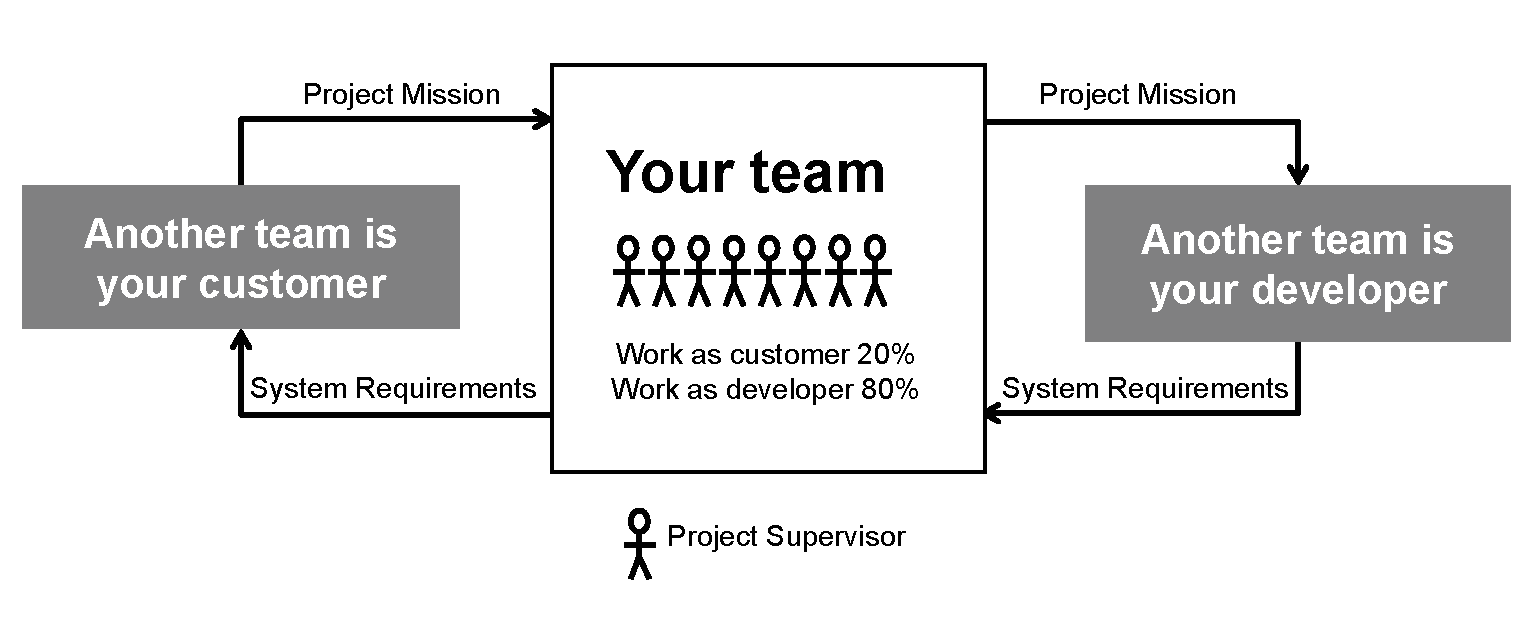
\includegraphics[scale=0.45]{fig/project-roles.eps}
%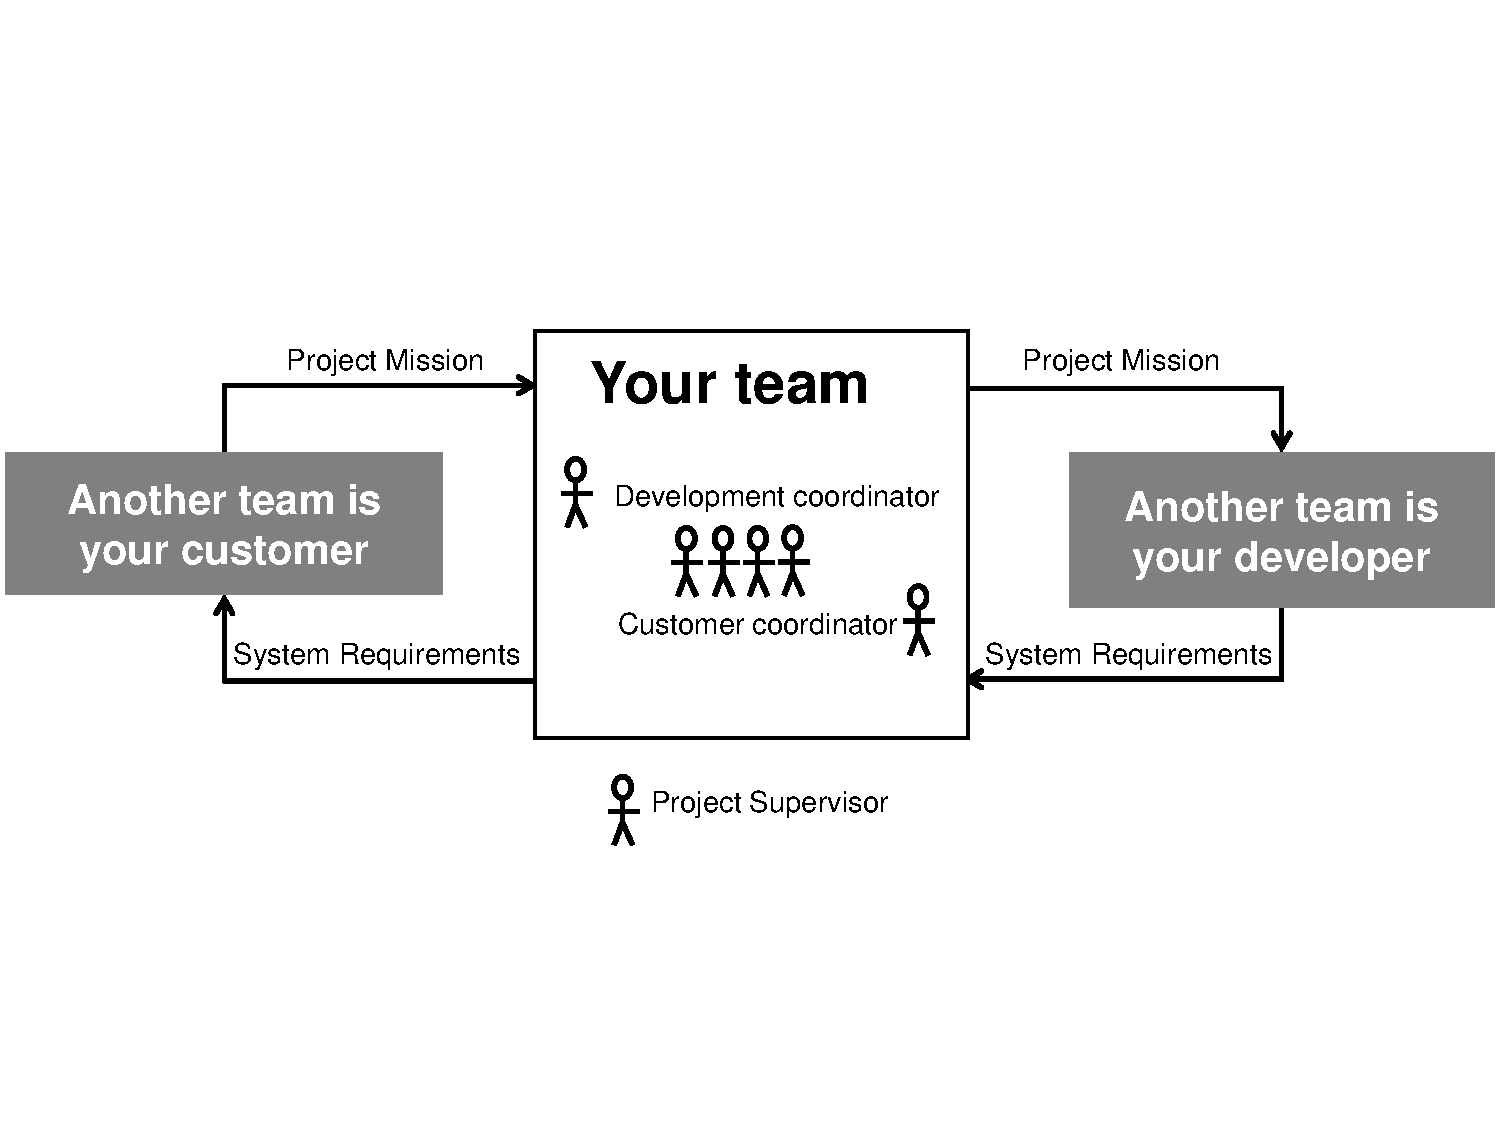
\includepdf[pages={1}]{fig/test2}
\begin{figure}[h]
\centering%trim = 1cm 1cm 2cm 1cm,clip,
\vskip-1.5cm
\hskip-2.9cm
%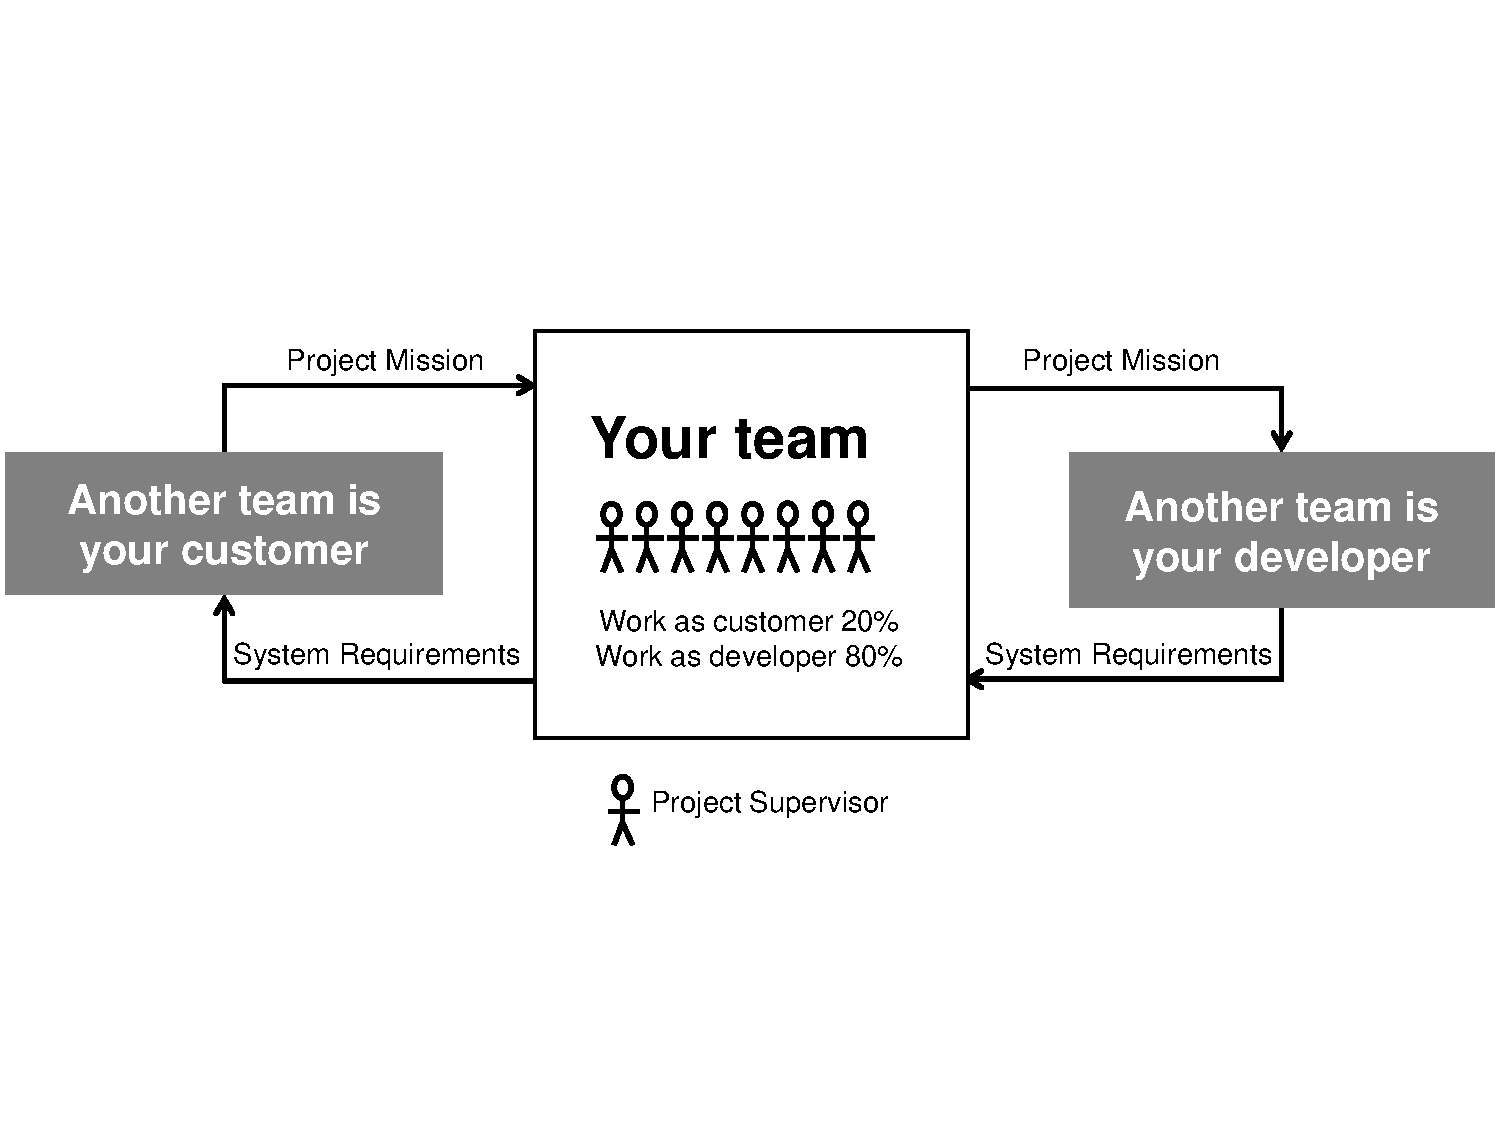
\includegraphics[trim = 5cm 6cm 1.5cm 10cm,clip,width=1.7cm]{fig/project-roles.pdf}
\vskip0.7cm
\end{figure}

\noindent Each project team has two different assignments:
\begin{description}[noitemsep]
\item[Customer work] (Kundarbete) To invent Project Mission v1 and act as customer providing domain expertise and feedback to another team that acts as developer.
\item[Development work] (Utvecklingsarbete) To develop a system model including requirements of different types at appropriate abstraction levels based on a given Project Mission from another team acting as your customer.
\end{description}

\noindent 
The project team consists of 6-8 members and these managers should be appointed among team members:

\begin{description}[noitemsep]
\item[P3RM] Project, Process, Prioritization, and Release Manager (1 person)
\item[SCCVM] Stakeholder, Customer Communication and Validation Manager (1 person) 
\item[TDEVM] Tools, Documents, Experiences and Version Manager (1-2 persons) 
\item [EPM] Elicitation and Prototyping Manager (1-2 persons) 
\item [QRM] Quality Requirements Manager (1 person)
\item [DRM] Data Requirements Manager (1 person)
%(om 2 personer får de redovisa hur de delar på ansvaret)
%\item[Development Coordinator] (Utvecklingskoordinator) This role is responsible for coordinating your team's requirements engineering work. This includes interacting with another team's customer coordinator. 
%\item[Customer Coordinator] (Kundkoordinator) This role is responsible for coordinating your team's work as customers and domain experts. This includes interacting with another team's development coordinator. 
\end{description}
The manager roles imply management, planning and coordination responsibilities, but managers should not do all the work: {\it all members should contribute in all parts!} 
\subsection{General project rules}
\begin{enumerate}[noitemsep]
\item The project comprises 80 hours per person.
\item Approximately 80\% of each team member's total effort should be devoted to development work.
\item Approximately 20\% of each team member's total effort should be devoted to customer work.
\item The total effort should be evenly distributed among participants.
\item In weeks W2, W4, and W6 a meeting should be scheduled with the project supervisor, where the project team reports on status, challenges and plans. 
\end{enumerate}

\subsection{Project deliverables}
\begin{tabular}{l |l p{5cm}  l}
{\it Phase} & {\it Deliverables} & {\it Deadline} \\
\hline
Definition & Project Mission v1& Week 1: Friday 09:00\\
Planning & Project Mission v2& Week 3: Monday 09:00\\
Iteration 1 & Release R1 & Week 4: Monday 09:00 \\
Iteration 2 & Release R2  & Week 6: Monday 09:00\\
   & Validation Checklist & Week 6: Monday 09:00\\
   & Validation Report & Week 6: Friday 09:00\\
Iteration 3 & Conference Presentation & Week 6: Sunday 15:00\\
   & Release R3 & Week 7: Sunday 23:59\\
   & Course Evaluation & Jan 30, Monday 09:00  \\

\end{tabular}
\vskip3mm

\noindent All deliverables should have a title, version number, team id (capital letter), system name and names of the project members. 

\subsubsection{Project Mission v1}

Acting as customer your team should prepare an initial version of a Project Mission for a development team. The Project Mission defines the system for which the employed project will elicit, prioritize, specify and validate requirements.

 \begin{enumerate}[noitemsep]
 \item The Project Mission should fit on {\bf one A4 page}, be in .pdf format for easy printing and web publishing. 
 \item The Project Mission should include a descriptive project name as well as the names of its authors.


\item You should fulfill the following criteria regarding the system you propose:
\begin{enumerate}[noitemsep,nolistsep]
\item You have a deep understanding of the application domain 
\item You have a genuine interest in the system 
\item You are be able to assess the value of detailed requirements 
\end{enumerate}
\item In the Project Mission you should take on the role of Key Customer. Your team then acts as one of many potential customer on an assumed market for the envisioned product. The development team owns the product and decides on priorities and product content, while your team gives input and provides feedback. which one of the following customer roles that you would like to play:
\end{enumerate}

\subsubsection{Project Mission v2}
Acting as developer your team should prepare a second version of the Project Mission where the scope of the project is further defined after dialog with your customer and supervisor. The purpose of this version is to act as an agreement that specifies what your team intends to develop, and what the customer can expect.
 
 \begin{enumerate}
 \item The Project Mission v2 is recommended to include the following information:
\begin{enumerate}[noitemsep,nolistsep]
\item Table of contents
 \item Background and other information from Project Mission v1 
 \item	Main goals and system context
 \item	Participants and potential stakeholders 
 \item	Description of planned activities and deliverables with deadlines
 \item	Diagram showing, per participant, the planned activities and time spent per week 
 \item	Responsibilities of project members 
\end{enumerate}

 \item With the above content it is useful if following questions can be answered:
 \begin{enumerate}[noitemsep,nolistsep]
 \item          What is the project about?
 \item          Who is participating in the project as members and as input providers?
 \item          What should be done in the project?
 \item          When should the results be delivered?
 \item          Who is responsible for what?
 \item          When shall who work with what?
 \item		What will the customer team spend their time on? 
\end{enumerate}
\end{enumerate}

\newpage
\subsubsection{Deliverables}
 \begin{enumerate}[nolistsep]
\item You should work iteratively and divide your work into 3 main iterations, each ending with a release with all your accumulated work products. (You  may have more sub-iterations with additional team-internal releases.)
\item The releases (delivered for the course) are denoted R1, R2 and R3.
\item For each release, the quality of your deliverables should represent a noticeable improvement.
\item Each release should be divided into two explicit parts: {\bf System Requirements} and {\bf Project Experiences}, each with its own {\bf table of contents}.
\item There should be an {\bf overview description} of each release to make navigation and assessment  easy, e.g. in a file called \verb+index.html+ or \verb+README.txt+.
\item A release \verb+Rn+ of team \verb+X+ should be delivered in {\it one single, self-contained} {\bf zip-file} named \verb+X-Rn.zip+ including {\it all} deliverables. If the file is too big to email then provide a http link to a downloadable zip-file.

\item Each deliverable may link to further resources such as html pages, pdf documents, screen images, text files, executables, etc., all contained in the delivered zip file. No external links outside the zip is allowed.

\item The last release R3 should include final versions of: System Requirements, Project Experiences, Validation Report \& Checklist (final versions by R2 also copied into R3), and Conference Presentation. Course Evaluation is delivered post course.

\begin{description}[noitemsep]
 \item[System Requirements] includes the following:  
  \begin{enumerate}[noitemsep]
 \item Different types of system requirements (e.g. data, function, quality) at different levels (e.g. goal, domain, product, design).
 \item Several specification techniques (e.g. context diagrams, features, virtual windows, task descriptions).
\item Each requirement should have a unique identity (name or number). 
 \item A subset of the requirements should be prioritized and release planned into the releases R3 (final course delivery), and (imagined future releases) R4 and R5. 
    \item  Design-level requirements are to be specified for the sub-set of requirements that are planned for release in R3 (see previous point). This sub-set of requirements shall be implemented as mock-up designs in the final course delivery (R3) using, e.g. screens and prototypes, analog drawings, clickable presentations, executable gui mockups. 
\end{enumerate}

 \item[Project Experiences] includes the following: 
   \begin{enumerate}[noitemsep]
   \item a description of your requirements engineering work, including experiences and reflections in relation to learning objectives.
 \item Description of the chosen methods/techniques for elicitation, specification, validation, and prioritization.
  \item Motivation for {\it why} you chose the used methods/techniques. 
 \item Reflection on  the usage of these methods/techniques in terms of what was successful and what was challenging. Example questions for reflection: What have you learned in relation to the learning objectives in this course program? What would you have done differently if you would do this project again as a ''real'' project, based on what you know now?  What have you learned in relation to the learning objectives?
 \item A personal statement by each team member that briefly explains each individual's contributions to the project results.
  \item The Project Experiences should {\it not} include course evaluation issues, but focus on your own work and learning outcome. 
  \end{enumerate}


\item[Validation Report] Acting as customer, you should validate release R2 from the other development team  and hand in your validation report together with your team's R2. Your team should produce relevant and useful issues for improvement. Each issue should be ranked for criticality.
 \item[Validation Checklist]  Acting as developer you should provide your customer with a requirements validation checklist tailored to the context.


\item[Conference Presentation]
Prepare and rehearse a short presentation.
   \begin{enumerate}[noitemsep]
 \item The total presentation time and further guidelines are given during the course.
 \item Spend approx. 10\% of the presentation time on the project's mission.
 \item Spend approx. 45\% of the time on project results and techniques used.
 \item Spend approx. 45\% of the time on experiences and learning outcome.
 \item Slides should be in \{.ppt|.pptx|.pdf\}.
\end{enumerate}


\item[Course Evaluation] (Not part of assessment.) A separate, free-form Course Evaluation document should be handed in by the team. If team members have different views, it is valuable if these differences are reflected. For each relevant course element (L, E, LAB, P, etc.) answer questions such as: What worked well?  If something needs improvement, {\it why} and {\it how} would you like it to be changed? 

 \end{description}
\end{enumerate}

\subsection{Project assessment}
\begin{enumerate}[noitemsep]
\item The deliverables Project Mission and Conference Presentation is pass/fail only.
\item The project grade of fail/3/4/5 is based on Release R3 and your Validation Report \& Checklist according to the criteria in the table on the next page: 

%\item Approx. $\frac{1}{2}$ of the grade is based on the {\bf System Requirements} in R3.
%\item Approx. $\frac{1}{3}$ of the grade is based on the {\bf Project Experiences} in R3.
%\item Approx. $\frac{1}{6}$ of the grade is based on the customer {\bf Validation Report} of R2.
\end{enumerate}

\newpage


\begin{sidewaystable}
\begin{adjustbox}{width=1.05\textwidth}
\begin{tabular}{| p{2.3cm} |p{5.5cm} | p{5.0cm} | p{5.7cm} |}
\hline
{\it Assessment area} & {\it Requirements for project grade {\bf 3}} \newline Demonstrate {\bf acceptable} ability to ... & {\it Also required for project grade {\bf 4}} \newline Demonstrate {\bf advanced} ability to ...& {\it Also required for project grade {\bf 5}} \newline Demonstrate {\bf excellent} ability to ... \\
\hline
\hline
{\bf Specification} & 
%3
	{\bf 3A)} apply more than one suitable specification technique (e.g. task descriptions and screen prototypes), and more than two types of requirement (e.g. data, function, quality), and more than three abstraction levels (e.g. goal, domain, product, design). \newline
	{\bf 3B)} define a system's boundaries and its interaction with external entities. \newline
	{\bf 3C)} reflect on specification experiences and reason about choices of specification methods in relation to different contexts. & 
%4	
	{\bf 4A)} combine different degrees of completeness and different levels of abstraction. \newline
	{\bf 4B)} use at least four different specification techniques adequately tailored to the context. \newline
	{\bf 4C)} provide explicit requirements rationale that reduce risks of misinterpretation. \newline
	{\bf 4D)} use hierarchies and requirements relations to manage evolving requirements structures. &
%5	
	{\bf 5A)} combine specification techniques in an explicitly motivated trade off between qualities and costs, where a high degree of specification completeness is achieved for a carefully selected subset of requirements. 	\newline
	{\bf 5B)} provide motivated estimations of target quality levels using well-defined scales. 
\\ \hline

{\bf Elicitation}  & 
	{\bf 3D)} apply more than one elicitation technique in a relevant way. \newline
	{\bf 3E)} reflect on elicitation experiences. &
	
	{\bf 4E)} reason about the need for further elicitation in relation to specification quality.& 

	{\bf 5C)} go beyond initial stakeholders and given frames, while challenging the domain boundaries and eliciting creative ideas and deep domain  knowledge in real-world contexts.
\\ \hline

{\bf Validation}  & 
	
	{\bf 3F)} to assess the quality of requirements and find relevant  problems of several different types. \newline
	{\bf 3G)} apply more than one validation technique. \newline
	{\bf 3H)} reflect on validation experiences.& 
	
	{\bf 4F)} to find, prioritize and discuss requirements quality problems of different types, while reaching beyond form issues. \newline
	{\bf 4G)} adapt the validation to the context and provide rationale for the chosen validation techniques. & 
	
	{\bf 5D)} reason about the relation between requirements quality problems and risks, both from a customer and developer viewpoint. \newline
	{\bf 5E)} utilize links among different types of specifications in validation efforts to find and address potentially harmful inconsistencies. \newline
\\ \hline

{\bf Prioritization}  & 
	
	{\bf 3I)} use more than one prioritization technique in a relevant way. \newline
	{\bf 3J)} reflect on prioritization experiences. &	
	{\bf 4H)} create a release plan for a subset of prioritized features, while taking into account precedence constraints. \newline
& 
	
%	{\bf 5G)} Demonstrate excellent ability to integrate and reflect on several prioritization techniques that are applied iteratively to different types of requirements. \newline
%	{\bf 5H)} Prioritization of quality requirements take different quality levels into account.  \newline
	{\bf 5F)} combine priorities from several stakeholders and use priorities and scheduling constraints to iteratively create a relevant release plan.\newline	   
	{\bf 5G)} use prioritization to focus improvements of specification quality and elicitation efforts for a well motivated subset of requirements.%, based on reflections on own experiences.
\\ \hline

\end{tabular}
\end{adjustbox}
\end{sidewaystable}

\end{document}
